% !TEX root = paper.tex
% !TEX encoding = UTF-8 Unicode
% -*- coding: UTF-8; -*-
% vim: set fenc=utf-8
% !TEX spellcheck = en-US
\section{Methods}
%------------------------------%
%: see Figure~\ref{fig:methods}
\begin{figure}[t!]%%[p!]
%\centering{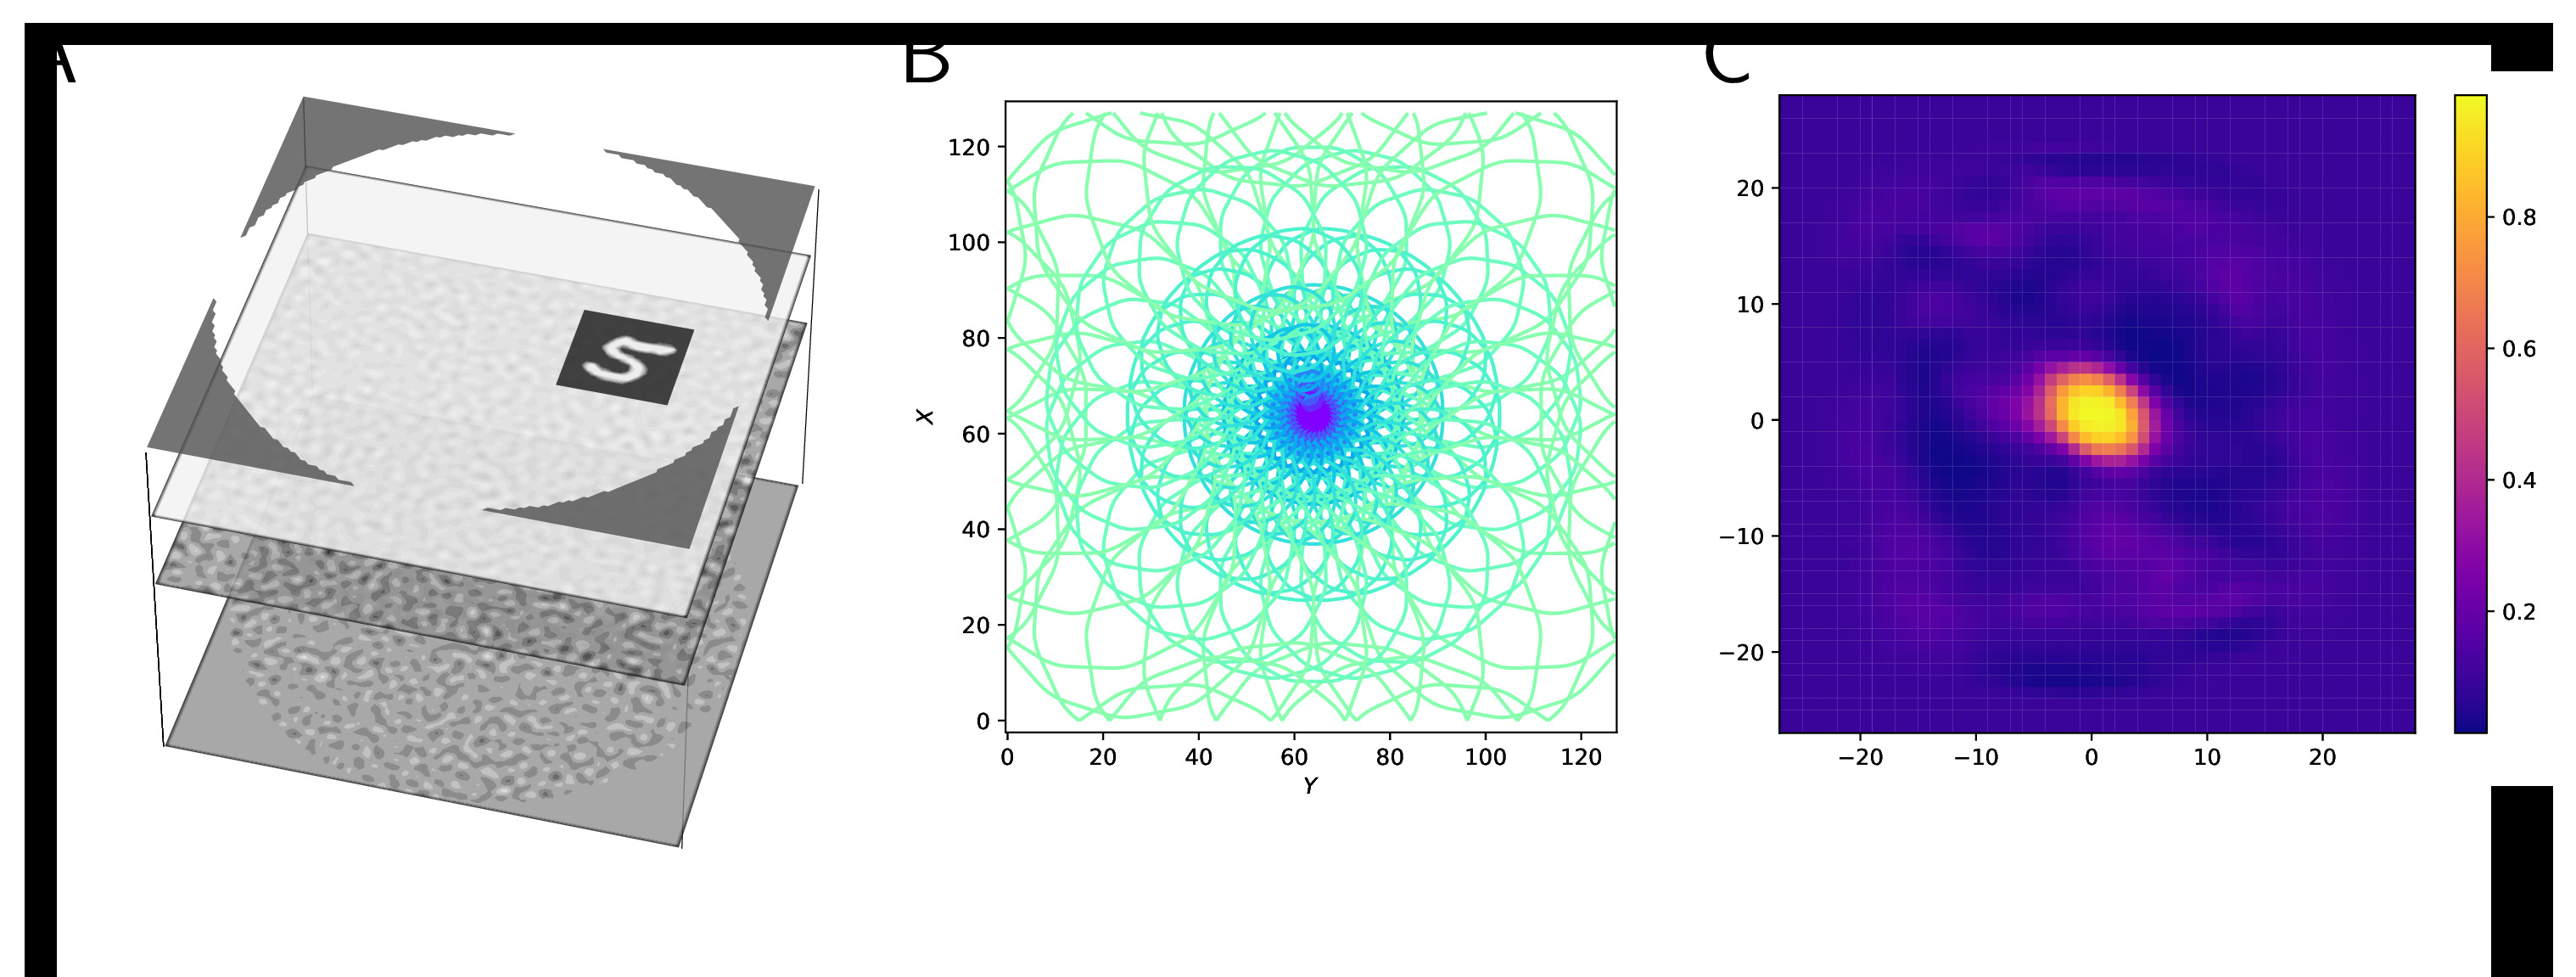
\includegraphics[width=\linewidth]{fig_methods}}
\caption{
{\bf Methods for simulating active vision}:
\A We first define the model which generates images. It is composed of different random processes: one choosing a sample image from the MNIST database (of size $28\times 28$) and placing it at a random position on the $128\times 128$ display. Then, this image is rectified and multiplied by a contrast factor and finally embedded in a natural-like noise with characteristics its contrast, mean spatial frequency and bandwidth~\citep{Sanz12}. %
\B The full-sized images are transformed into a retinal image which will be fed to the ``where'' pathway. This is implemented by a bank of filters whose centers are centered of a log-polar grid and whose radius increases proportionally to eccentricity. Crucially, a similar transform is used to compute the accuracy of each hypothetical saccade, as represented by the collicular map. %
\C The ``where'' pathway is implemented by a three-layered neural network consisting of the retinal input, two hidden layers with $1000$ units each and a collicular output. Each unit is associated with a ReLU non-linearity. To learn to associate the output of the network with the ground truth, supervised training is performed using back-propagation with a binary cross entropy loss which measure the distance between both distributions. The network learns in about 20 epochs as shown by the decrease of the loss function. Overlaid is the associated accuracy of the full active agent. This is computed by classifying the foveal image using the ``what'' pathway, after centering the gaze using the result of the ``where pathway''. This shows a gradual increase in accuracy from the baseline ($10\%) to approximately an average of $XX\%$. %
}%
\end{figure}%
%%------------------------------%

\subsection{Principles}
A current hypothesis regarding active vision is that visual scenes most often consist of a single visual object of interest.
The visual scene is here made of a foreground (the target) and a noisy background. An agent controls a focal visual sensor that can move over the visual scene through saccades.


%The target accuracy map is also organized radially in a log-polar fashion, making the target position estimate more precise at the center and fuzzier at the periphery. This modeling choice is reminiscent of the approximate log-polar organization of the superior colliculus (SC) motor map {\bf[TODO:REF]}.
%This retinotopic organization is preserved along the visuo-motor pathway as expected from observations {\bf[TODO:REF]}.


%<<<<<<< HEAD
%A second simplifying assumption is that the putative effect of a saccade should be condensed in a single number, the \emph{accuracy}, that is a statistics over the (scene understanding) benefit obtained from past saccades in the same context, independently of the identity of the visual objects. In detail, the primary visual information should be transformed so as to predict how accurate the categorical classifier will be after the saccade is carried out~\citep{Dauce18}. The set of all possible saccade predictions should form an \emph{accuracy map}.
%An accuracy map abstracts here a full sequence of operations, including (i) an initial visual examination, followed by (ii) a decision, (iii) a saccade realization and a (iv) second visual examination that should finally (v) determine the category of the target. 
%It should be mostly organized radially, preserving the initial retinotopic organization, with high predicted accuracies reflecting a high probability of target presence at given locations. 
%Such  a \emph{predictive accuracy map} is assumed to be the cornerstone of a realistic saccade-based vision system, with action selection (motor map) overlaying the accuracy map through a winner-takes-all mechanism (as thought to be done in the superior colliculus). Of course, each different initial visual field comes with a different accuracy map (essentially conveying information about the target retinotopic position).
%Our main argument is that such an accuracy map is trainable in a rather straightforward way, through trials and errors, by actuating saccades after processing the visual input, and taking the final classification success or failure as a teaching signal. 
%\fi
%=======

Active inference assumes a hidden emitter $e$, which is known indirectly through its effects on the sensor, that obey to a generative process : $x\sim p(X|e)$. The real emitter state $e$ being hidden, a parametric model $\theta$ is assumed to allow estimate the cause of the current visual field through model inversion thanks to Bayes formula, in short:
$$p(E|x) \propto p(x|E;\theta)$$
with $x$ the visual field in our case. Assume now that the cause $e$ of the visual field splits in two (independent) components, namely $e = (u,y)$ with $u$ the body posture (in our case the gaze orientation) and $y$ the object shape (or object identity). Assume also that a set of motor commands $A = \{..., a, ...\}$ may control the body posture, but not the object's identity, so that $y$ is invariant to $a$.
Then, before taking a decision, the consequence of every saccade should be analyzed  through model inversion \emph{over the future observations}, that is predicting the effect of every $a$ in $A$ to choose the action that may optimizes future inferences. The benefit of each $a$ is quantified through a certain metric (future accuracy, future posterior entropy, future variational free energy, ...), that depend on the current inference $p(U,Y|x)$. Each saccade $a$ is thus expected to provide a new visual sample from a given scene statistics, which may increase the understanding of the scene (here the target position and category). However, estimating the effect of every action over the range of every possible object shapes and body postures is combinatorially hard, even in simple cases such as vision, and thus infeasible in practice. 


%Though the effect of action is too complex to be inferred from a generative model, we assume here that it is trained by sampling, i.e. by "trial and error".

There are however many shortcuts allowing to render the calculation amenable. This includes (i) sparse encoding, (ii) approximate inference through model separation, and (iii) sampling-based metric training. 

\paragraph{Sparse encoding}
First, both the visual features and the expected target position may to be expressed in log-polar coordinates. On the primary visual side, local visual features (first and second order orientation filters) are radially organized around the center of fixation, with small and tightened receptive fields at the center and more large and scarce receptive fields at the periphery. The issued observation vector $\boldsymbol{x}$ compresses the original image by about 90\%, with high spatial frequencies preserved at the center and only low spatial frequencies conserved at the periphery.

\paragraph{Approximate inference}
Second, we %start as in~\citep{Friston12} by a probabilistic formulation, and 
use the fundamental hypothesis outlined in Figure~\ref{fig:intro}: the position of an object is independent from its category.  This allows considering $u$ and $y$ being independently inferred from the current visual field, i.e $p(U,Y|x) = p(U|x) p(Y|x)$. This property is strictly true in our setting and is very generic in vision for simple classes (such as digits) and simple displays (but see~\citep{Vo12} for more complex visual scene grammars). 
From this independence hypothesis, we may separate both inferences (identification vs localization) in two separate pathways with different morphologies (respectively foveal and peripheral). Note that from the retinotopic projection of the visual information, this independence is conditional on action: both pathways should update their beliefs upon decisions made in each respective pathway.
%A first simplifying assumption is a separation of the position and category inferences in two separate pathways, namely the ``What'' and the ``Where'' pathways.
The agent visual categorical pathway (the ``What'' pathway) is supposed to be realized by the known ``LeNet'' classifier~\citep{Lecun1998}, that processes the $28 \times 28$ central pixels to identify the target category (see dashed red boxes in  Figure~\ref{fig:intro}-C). This central classifier displays a high accuracy at the center, and a fast decreasing accuracy with target eccentricity, as shown in figure \ref{fig:results}-D. In contrast, the visual orientation pathway (the ``Where'' pathway) takes the full visual field into account in order to tell whether a target is present at the different peripheral locations, in order to monitor future saccades.

As for the modelling of the ``what'' pathway, we used the implementation of LeNet by invited Leann 3 which is provided by the pytorch library~\citep{Paszke17}. This 3-layered Convolutional Neural Network is trained over the MNIST database after approx $20$ training epochs. It achieves an average $98.7\%$ accuracy on the test dataset. In particular, we could also evaluate after this  training phase the accuracy map of the classifier knowing a translational shift imposed to the input image. 



\paragraph{Metric training}
Third, the putative effect of every saccade should be condensed in a single number, the \emph{accuracy}, that is the expected benefit of issuing saccade $a$ %regarding the target identity, both assuming $p(U|\boldsymbol{x})$ and $p(Y|\boldsymbol{x})$ 
from the current observation. Taking $a$ a possible saccade and $\tilde{\boldsymbol{x}}$ the corresponding future visual field, the result of the categorical classifier over $\tilde{\boldsymbol{x}}$ can either be correct (1) or incorrect (0). 
If this experiment is repeated many times over many visual scenes, the probability of correctly classifying the future visual field $\tilde{\boldsymbol{x}}$ after a saccade $a$ forms a probability, i.e. a number between 0 and 1, that reflects the proportion of correct and incorrect classifications.
% when issuing a saccade $a$ after seeing $\boldsymbol{x}$ (the initial visual field). 
It more or less corresponds to checking the true target identity $\hat{y}$, i.e. $p(\hat{y}|\tilde{\boldsymbol{x}})$, including the update of the eye direction $\tilde{u}$, that is a sample of the ``real'' generative process. Active inference thus needs $y$ and $u$ to be (at least partly) readable from the present view, in order to effectively predict future inferences, which is possible but computationally intensive.   
Instead of inverting a generative model, better off is to form a statistics over the (scene understanding) benefit obtained from past saccades in the same context, that is forming an \emph{accuracy map} from the current view. This is the essence of \emph{sampling-based metric prediction}.

In detail, the primary visual field should be transformed so as to predict how accurate the categorical classifier will be after the saccade is carried out~\citep{Dauce18}. %The set of all possible saccade predictions should 
An accuracy map abstracts here a full sequence of operations, including ($i$) an initial visual examination, followed by ($ii$) a decision, ($iii$) a saccade realization and ($iv$) a second visual examination that should finally ($v$) determine the category of the target.
It should be mostly organized radially, preserving the initial retinotopic organization, with high predicted accuracies reflecting a high probability of target presence at given locations.
Such  a \emph{predictive accuracy map} is assumed to be the core of a realistic saccade-based vision system, with action selection (motor map) overlaying the accuracy map through a winner-takes-all mechanism (as thought to be done in the superior colliculus). Of course, each different initial visual field comes with a different accuracy map (essentially conveying information about the target retinotopic position).
Our main argument is that such an accuracy map is trainable in a rather straightforward way, through trials and errors, by actuating saccades after processing the visual input, and taking the final classification success or failure as a teaching signal.

\subsection{Implementation}
To check this hypothesis, we train a multi-layer neural network to predict accuracy maps from a retinotopic log-polar encoding of the visual image. 

\paragraph{log Polar encoding}

\paragraph{Background noise setting}

\paragraph{Classifier training}
Modern parametric classifiers are composed of many layers (hence the term ``Deep Learning'') that can be trained through gradient descent over arbitrary input and output feature spaces  {\bf [REF?]}. The ease of use of those tightly optimized training algorithms allow to quantify the difficulty of a task through training failure or success. Consider the visual features  $\boldsymbol{x}$ as the input and a logpolar retinotopic vector $\boldsymbol{a}$ made of $n$ Bernouilli probabilities (success probabilities) as the output. A textured background noise is used at the input so that (i) the target statistics should barely differ from that of the background and (ii) a  categorical classifier may not be trainable with the initial view as the input. A training set is made of randomly generated noisy images, with a low-contrast $28\times 28$ MNIST character   {\bf [REF?]} randomly positioned around the center of fixation (at maximum $30$ pixels from the center of fixation). The images are first whitened  {\bf [REF?]}, and then transformed through $16384$ oriented log-polar filters radially organized around the center of fixation, with tight receptive fields at the center and large receptive fields at the periphery. The filters are organized in $10$ spatial eccentricity scales (respectively placed at around $2$, $3$, $4.5$, $6.5$, $9$, $13$, $18$, $26$, $36.5$ , and $51.3$ pixels from the center), and $16$ angular directions, allowing them to cover most of the original 128 $\times$ 128 image. Each visual input is accompanied with a corresponding accuracy map also organized radially through $10$ eccentricity scales and $16$ peripheral directions. The training is done in Pytorch  {\bf [REF?]}. The parametric neural network is made of two fully connected hidden layers of size $1000$, with ReLu activation and $50 \%$ drop-out on the last layer. The network is trained over $600,000$ saccades on full-images, using the binary cross-entropy loss as the error signal, with a learning rate equal to $10^{-4}$. The training is done in about 3 hours on a laptop.


